%% Template for a preprint Letter or Article for submission
%% to the journal Nature.
%% Written by Peter Czoschke, 26 February 2004
%%

\documentclass{nature}
%\documentclass[12pt]{article}

%% make sure you have the nature.cls and naturemag.bst files where
%% LaTeX can find them

\bibliographystyle{naturemag}

\usepackage{graphicx}
\usepackage{amssymb,amsfonts,amsmath}
\usepackage{subfigure}
\usepackage{stfloats}


%% OPTIONAL MACRO DEFINITIONS
\def\s{\sigma}
\newcommand{\be}[0]{\begin{equation}}
\newcommand{\ee}[0]{\end{equation}}
\newcommand{\lb}[0]{\left(}
\newcommand{\rb}[0]{\right)}


\title{Arctic sea-ice loss and cold Eurasian winters in the face of internal variability}% 81char

%% Notice placement of commas and superscripts and use of &
%% in the author list


\author{Kelly E. McCusker,*$^{1,2}$ \& John C. Fyfe,$^{2}$ \& Michael Sigmond$^2$}

% NatGeo requirements:
% Title If possible, the title should give a sense of the main new finding, and should not exceed 90 characters, including spaces. Nature Geoscience titles do not contain technical terms or abbreviations unless absolutely necessary. We strongly discourage punctuation or active verbs.@@
% Letter 2,000 words no methods, 3 figures
% Article 3,000 words no methods, include section titles, 6 figures. No refs in abstract. ~500 words of Intro. 1-2 para of conclusions


\begin{document}

\maketitle

\begin{affiliations}
 \item School of Earth and Ocean Sciences, University of Victoria, Victoria, BC, V8P 5C2, Canada
 \item Canadian Centre for Climate Modelling and Analysis, Environment Canada, Victoria, BC V8W 2Y2, Canada
\end{affiliations}


\begin{abstract}
Arctic sea ice loss has been implicated in the recent trend toward unusually cold Eurasian winters \cite{liu12,mori14,kim14}. Whether the linkage follows from anthropogenic sea ice loss, however, remains an open question as the sea-ice loss combines anthropogenic response and internal (random) variability \cite{swart15,wettstein14} and because of confounding wintertime variability over the Eurasian continent \cite{deser12b,screen14a}. Here, we isolate the anthropogenic and random components of the linkage using a large ensemble of atmosphere-only model simulations with prescribed sea ice loss taken from simulations of the companion atmosphere-ocean-cryosphere model and from observations. We find no evidence of a sea-ice loss related decrease in Eurasian winter temperature. However, we do find long periods of winter Eurasian cooling linked to internally-generated circulation features over the Barents and Kara Seas regions of the Arctic. These results challenge the perception that Arctic sea ice loss was responsible for the recent prevalence of unusually cold Eurasian winters, showing instead that these winters were more likely the consequence of internal variability, with implications for our understanding of impacts and adaptation in human and natural high-northern latitude systems. 
\end{abstract}

Global average surface air temperatures in the boreal cold season have been rising faster than the long-term annual average \cite{wallace12} and exhibit further enhanced warming over the Arctic in part due to positive feedbacks related to sea-ice loss \cite{screen10,cohen14}. Epoch differences of winter (December-January-February; DJF) surface air temperature (SAT) between 2002-12 and 1979-89 reveal warming upward of 2$^\circ$C over the polar cap, collocated with areas of sea ice loss (Figure \ref{fig:fig1}a). Contemporaneous cooling of greater than 1$^\circ$C over the Eurasian continent in winter is also evident; a feature that is particularly striking when considered in the context of broad hemispheric warming, which can in part be attributed to anthropogenic forcing \cite{gillett08,qian15}. 

Since the year 2000, there have been a greater number of Eurasian winters exhibiting increasingly cold anomalies, especially in relation to the evolution of northern hemisphere temperature; Figure \ref{fig:fig1}b shows Eurasian winter SAT with northern hemisphere average temperature removed. The difference of Eurasian SAT between epochs marked in gray shading in Figure \ref{fig:fig1} (-1.1$^\circ$C) is statistically significant at the 90\% level (p=0.09), indicating that Eurasian SAT has deviated a significant amount from expected general hemispheric warming. Coincident with these cold anomalies, large reductions in autumn and winter Arctic sea ice area have occurred, particularly in the Barents and Kara Seas (BKS) sector (along the western half of the Russian coastline; Figure \ref{fig:fig1}c). The epoch difference in sea-ice area (SIA; -0.3e$^6$ km$^2$) is also statistically significant (p$<$0.001). Observationally-based studies using correlation and composite analyses confirm a positive correlation between Barents \cite{inoue12} or Kara \cite{outten12} Seas sea ice concentration (SIC), and implicate the former in initiating the latter through a weakened meridional temperature gradient and ensuing changes in circulation and cyclone track. However, the observed relationship of BKS turbulent heat flux to Eurasian SAT suggests atmospheric variability, not sea ice loss, drives both \cite{sorokina15}. 

The direction of causation in observationally-based studies remains a challenge, but modeling studies in which the influence of a change in sea ice is isolated provides some support for the hypothesis that BKS sea ice loss can initiate Eurasian cooling through a Rossby wave-train emanating out of the BKS region, incited by turbulent heat flux from the increased area of open water \cite{honda09,petoukhov10,mori14,kim14,peings14}. However, the magnitude of the modelled effect is weak compared to the observed Eurasian cooling, and the timing and placement of the cold anomaly is not consistent. Furthermore, still other studies point to sea surface temperature (SST) changes in the North Atlantic or @@ as a possible root sources of Rossby wave propagation and Eurasian cooling (cite@@). Further clarification of the link between sea ice loss in the Barents-Kara Seas and Eurasian SAT anomalies is thus warranted. Here we address whether a long term (1979 - 2012) decrease of Barents-Kara sea ice concentration in winter is not only associated with, but is the cause of a decrease in Eurasian winter SAT over this time period (Figure \ref{fig:fig1}). We take into account the powerful influence of internal variability of the climate system, as well as the imprint of internal variability on the change in sea ice itself. 

We do this by analysing the relationship of multi-decadal changes in SIA to multi-decadal changes in SAT in coupled simulations and in atmosphere-only simulations with prescribed sea ice loss. The coupled simulations consist of a fifty-member large ensemble (LE) of Canadian Earth System Model version 2 (CanESM2 ref@@) simulations with historical forcing as well as a 1,000 year CanESM2 preindustrial control simulation with no forcing. Each CanESM2 historical realization is run with identical historical forcings with slightly varied initial conditions, so we use the LE to characterize the impact of external forcing and internal variability on multi-decadal changes in SIA, Eurasian SAT, and their relationship on a multi-decadal timescale. In comparison, the relationships uncovered in the preindustrial simulation are due only to internal variability. The historical LE results are presented as epoch differences between 2002-12 and 1979-89 for each realization, which we refer to as ``CGCM", while the preindustrial control is segmented into 11-year climatologies and randomly sampled to generate a set of fifty anomalies, which we refer to as ``Preindustrial" (see Methods). 

The general hypothesis is that a decrease in sea ice concentration initiates local warming that leads to changes in circulation that cause Eurasian wintertime cooling (@@cite). We start by examining the first link in the chain, the change in Arctic SIA. The average DJF Arctic SIA anomaly in Preindustrial is approximately zero, whereas it is -1.2 million km$^2$ in CGCM due primarily to anthropogenic forcing over this time period. Yet, even on this multi-decadal timescale, internal variability produces a range of anomalies that span nearly one million km$^2$ in CGCM and over one million km$^2$ in Preindustrial (Supplementary Figure \ref{fig:supfig1}), consistent with previous findings \cite{swart15}. The observed value (-0.78 million km$^2$), derived from satellite measurements by the National Snow and Ice Data Center (NSIDC), is encompassed only by the 2.5-97.5\% range of CGCM anomalies and not by Preindustrial anomalies, consistent with the presence of a human influence on observed sea ice loss \cite{min08}. Meanwhile, the forced response of Eurasian SAT is to warm, as seen in the average of CGCM Eurasian SAT anomalies in gray in Figure \ref{fig:fig2}. The majority of these CGCM anomalies are positive, with a probability of cooling of just p=@@. Thus, Eurasian SAT is dominated by anthropogenic forcing in CGCM, with a rare occurrence of a long-term cooling trend. This, despite having sea ice loss in the Arctic and in the Barents/Kara seas comparable in magnitude to observations. However, is it possible that changes in sea ice play a role in modulating Eurasian SAT?

To isolate the impact of Arctic sea ice loss on Eurasian SAT, we execute pairs of 120-year atmosphere-only simulations with prescribed ``past" (1979-89) and ``present day" (2002-12) SIC, SST, and sea ice thickness (SIT) taken from five members of CGCM (see Methods). The Arctic SIA anomalies prescribed are shown as gray circles in Supplementary Figure \ref{fig:supfig1} in the context of CGCM SIA anomalies. These atmosphere-only results, which we refer to as ``AGCM", are presented as anomalies between present-day and past simulations, and are sub-sampled into fifty 11-year averages to mimic CGCM. Thus, AGCM anomalies are due to the loss of Arctic sea ice, and to internal variability. We find that sea ice loss in isolation does not cause a systematic Eurasian winter cooling (Figure \ref{fig:fig2}); the average of fifty 11-year anomaly periods is approximately 0$^\circ$C, with a probability of a cold anomaly of p=@@. [@@long-term averaging here?] Moreover, Eurasian SAT showed nearly identical behaviour in an additional atmosphere-only ensemble of timeslice simulations in which boundary conditions were held fixed for 600 years of simulations (``AGCM\_fixed"; see Methods and Supplementary Figure @@). These SAT anomaly distributions are similar to that of Preindustrial, indicating that the multi-decadal SAT variations in AGCM are simply dictated by internal variability.   %what would be expected of Eurasian SAT due solely to internal variability in an unforced simulation %The influence of the differences in the sea ice boundary conditions is indistinguishable from internal variability (Supplementary Information) and so we do not attempt to separate their contributions further.

To understand further what drives Eurasian SAT, we examine the relationship in CGCM and AGCM of changes in Eurasian SAT to changes in geopotential height at 500 hPa (Z500), which we use as a proxy for circulation, averaged over the important Barents/Kara seas region. Figure \ref{fig:fig3} shows ellipses encompassing 95\% of simulated CGCM and simulated AGCM BKS Z500 and Eurasian SAT anomalies, along with linear regression lines. As Z500 anomalies over the Barents-Kara Seas increase, Eurasian SAT anomalies robustly decrease in CGCM (r$^2$=0.17; p=0.003) and AGCM (r$^2$=0.66; p$<$0.0001). Thus, the physical mechanisms that lead to cooler Eurasian SAT are consistent with existing work that implicates an anomalous anti-cyclone over the Barents-Kara Seas region \cite{honda09,petoukhov10,mori14}. The regression slopes are nearly identical in the externally-forced coupled (CGCM) and sea-ice-loss uncoupled (AGCM) simulations (-0.2$^\circ$C / 10m and -0.3$^\circ$C / 10m, respectively), suggesting that the relationship is not a distinct feature of coupling, or of external forcing. Furthermore, AGCM\_fixed exhibits a similar relationship (slope=0.2$^\circ$C / 10m; r$^2$=0.24; p$<$0.001) even with a fixed Arctic sea ice anomaly (Supplementary Figure @@), which points towards Eurasian SAT anomalies being driven by internally-generated circulation features and not BKS sea ice anomalies. Further support for this theory comes by way of BKS Z500 and Eurasian SAT changes composited on high and low BKS SIC anomalies, shown as plus symbols in Figure \ref{fig:fig3}. The change in Eurasian SAT composited on the bottom 10 BKS sea ice anomalies (``low" relative sea ice concentration) in CGCM is not significantly different from the change in Eurasian SAT composited on the top 10 BKS sea ice anomalies (``high" relative sea ice concentration) in CGCM (p=@@). Likewise, the changes in Eurasian SAT composited on high and low BKS SIC in AGCM are not significantly different from one another (p=@@). Recall that AGCM has 5 different sea ice boundary conditions total, so the AGCM composite is made up of ten 11-year anomaly periods subsampled from the simulation with the greatest amount of sea ice (high) and subsampled from the simulation with the smallest amount of sea ice (low). @@observed val... @@weak relationship b/c sic and z500 %Note that the AGCM composite is made up of ten 11-year anomaly periods subsampled from the simulation with the greatest amount of sea ice (?high?) and subsampled from the simulation with the smallest amount of sea ice (?low?), because AGCM has just 5 different sea ice boundary conditions total.

We have 

%compute composites based on high and low anomaly values of various regionally-averaged variables

%A key question remains; To However, this mechanism does not hinge on sea ice concentration, as will be shown next. %@@ check the E sims relationship again and say something about that?
%The smaller variance explained in CGCM is likely due to the external forcings at play, however the slopes of the regression lines in CGCM and AGCM are nearly identical, suggesting that the relationship is not a distinct feature of external forcing.

%High BKS Z500 height anomalies are associated with cold Eurasian SAT anomalies and vice versa. This relationship is consistent with the notion proposed by others that high geopotential height (or sea level pressure) over areas of sea ice loss in the Barents/Kara Seas is associated with colder Eurasian winters (cite@@). The linear relationship is highly significant in both ensembles (p$<$0.01), however the variance explained by the relationship in AGCM is greater (r$^2$=0.65 compared with r$^2$=0.17 for CGCM), most likely due to the external forcings at play in CGCM. However, the slopes of the regression lines in CGCM and AGCM are nearly identical, suggesting that the relationship is not a distinct feature of sea ice loss. % (changes in greenhouse gases, tropospheric aerosols, as well as occasional volcanic eruptions, for example) % @@ DO PI relationship

%These relationships describe how multi-decadal changes in Eurasian winter SAT vary with multi-decadal changes in circulation, rather than the more standard technique of examining relationships on an inter-annual timescale. In the case of AGCM, there is no additional forcing The red circle shows the observed value. 

%What is novel here, however, is that there is no indication that changes in sea-ice concentration are the fundamental origin of Eurasian SAT anomalies because sea-ice concentration is prescribed in our simulations. 

%, plus five additional 120-year simulation pairs with the average of the five CGCM members past and present-day boundary conditions. %We find that in DJF, the SAT anomalies produced by variable sea ice loss versus average sea ice loss are indistinguishable from one another due to the strong influence of internal variability (Supplementary Info@@). Therefore, we present results from the variable boundary condition simulations only, which we refer to as ``AGCM". These results are presented as anomalies between present-day and past simulations, and sub-sampled into 11-year averages to mimic CGCM.



%Could it be that the cold side of the Eurasian SAT distribution is related to greater amounts of BKS sea ice loss?

%CGCM shows no propensity toward multi-decadal Eurasian winter cooling, despite  %The observed cold anomaly falls just outside the range of CGCM (Figure \ref{fig:fig2}), suggesting that observed Eurasian cooling is particularly exceptional, despite unexceptional observed sea ice loss. 
% @@ OPTIONS: get into the next figure describing the physical connection b/w cold eurasia and goepotential height, including composites. OR: introduce AGCM simulations and say how there is no systematic warming or cooling due to sea ice loss. so far I kind of like option 1.

%Eurasian SAT anomalies in CGCM are generally positive, with a probability of cooling of just p=@@. The forced response of Eurasian SAT is to warm
% @@ shorten to just say something like: the observed value of sea ice loss is captured by the 2.5-97.5 confidence range of CGCM, but not Preindustrial (supp fig). This is consistent with the presence of a human influence on observed sea ice loss \cite{min08}; by our estimate, 36\% of observed ice loss is due to internal var (supp info) etc @@


%We further clarify the specific role of sea ice loss in isolation by executing an ensemble of so-called `timeslice' simulations with the companion atmosphere-only model, CanAM4 (ref@@) (see Methods).

%In order to estimate the impact of isolated sea ice loss on Eurasian SAT, we execute pairs of 120-year atmosphere-only simulations with prescribed ``past" (1979-89) and ``present day" (2002-12) SIC, SST, and sea ice thickness (SIT) taken from five members of CGCM (see Methods and Supplementary Figure \ref{fig:supfig1}), plus five additional 120-year simulation pairs with the average of the five CGCM members past and present-day boundary conditions. We find that in DJF, the SAT anomalies produced by variable sea ice loss versus average sea ice loss are indistinguishable from one another due to the strong influence of internal variability (Supplementary Info@@). Therefore, we present results from the variable boundary condition simulations only, which we refer to as ``AGCM". These results are presented as anomalies between present-day and past simulations, and sub-sampled into 11-year averages to mimic CGCM.


%The five sets of boundary conditions sample different representations of internal variability in the sea ice anomaly. Additionally, we execute five pairs of 120-year AGCM simulations with prescribed boundary conditions that are the average of the 
%, however, we determined that the sensitivity to sea ice boundary forcing is overpowered by internal variability in winter and outside the Arctic (see Supplementary Info@@). %and internal variability 

%The average DJF Arctic SIA anomaly in CGCM, which can be interpreted as the sea ice loss due to external forcing, is equal to -1.2 million km$^2$ with an anomaly range due to internal variability that encompasses the observed value from the National Snow and Ice Data Center (NSIDC; Supplementary Figure \ref{fig:supfig1}).

%Internal variability generates a wide range of DJF sea ice anomalies (approximately 1 million km$^2$, compared with a mean anomaly of -1.2 million km$^2$; Supplementary Figure \ref{fig:supfig1}).

%In order to estimate the impact of just sea ice loss and internal variability on changes in SIA and Eurasian SAT, we execute pairs of 120-year AGCM simulations with prescribed ``past" (1979-89) and ``present day" (2002-12) SIC, SST, and sea ice thickness (SIT) taken from the five CanESM2 Historical simulations (Supplementary Figure \ref{fig:supfig1}) that were submitted to the Climate Model Intercomparison Project 5 (CMIP5). We present AGCM results as anomalies between present-day and past simulations, and sub-sampled into 11-year averages to mimic CGCM.



%Human influence on observed Arctic sea ice extent is clear \cite{min08}, however internal variability also makes a strong imprint on sea ice extent (Ref \cite{swart15} and Supplementary Figure 2), up to 47-57\% of observed September extent \cite{stroeve07,kay11}.

%; up to 40\% of the magnitude of winter sea ice loss, by our estimate using the LE (see Supplementary Figure 2 and Supplementary Info), and up to 47-57\% in Autumn by other measures \cite{stroeve07,kay11}. 


%Because each CGCM realization is run with identical historical forcings with slightly varied initial conditions, we can use the LE to characterize the impact of external forcing and internal variability on multi-decadal changes in SIA and Eurasian SAT. To do this, we take epoch differences between 2002-12 and 1979-89 for each realization, and compute composites based on high and low anomaly values of various regionally-averaged variables (see below). Similarly, we construct an analogous ensemble of AGCM simulations in which  

% OR: Modelling studies that isolate the effect of sea ice loss on the atmosphere yield varying degrees of support for the hypothesis
% check what time-resolution these studies look at: are they multi-decadal trends or inter-annual? @@

 
 
 
 =================== OLD BELOW ==========================
 
 However, while human influence on observed Arctic sea ice extent is clear \cite{min08}, interpretation of this Arctic sea ice--Eurasian SAT connection as an anthropogenic signal is limited by the strong imprint of internal variability on observed sea ice loss itself \cite{swart15}. 

To estimate the anthropogenic component of observed winter sea-ice loss, we examine a distribution of DJF sea ice loss between the periods (1979-89) and (2002-12) in a large ensemble (LE) of 50 Historical simulations executed in the Canadian Earth System model version 2 (CanESM2; Figure \ref{fig:fig2}). The average of the distribution represents the anthropogenically-forced sea ice area anomaly, while each individual realization represents one version of an ``observation", displaced from the average by some amount due only to internally-generated variability. Here internal variability generates a range in DJF sea ice loss over this time period of approximately 1 million km$^2$. 

An estimated upper bound on the contribution of internal variability to a sea-ice area anomaly can be made using the extreme end-points of the distribution in Figure \ref{fig:fig2}: taking the minimum ice anomaly (-1.7e$^6$ km$^2$) distance from the distribution average (-1.2e$^6$ km$^2$), we find that internal variability can account for up to 40\% of the historical sea-ice area anomaly: (-1.7e$^6$ - (-1.2e$^6$))/-1.2e$^6$ = 0.39 or about 40\%. Similarly, the maximum ice anomaly (-0.7e$^6$ km$^2$) gives approximately 40\%. The true observed DJF Arctic sea-ice area anomaly derived from satellite measurements by the National Snow and Ice Data Center (NSIDC) is encompassed by the Historical LE (Figure \ref{fig:fig2}) and indicates a similar contribution from internal variability (36\%), somewhat smaller than alternative calculations that equal 47-57\% for September sea ice trends \cite{kay11,stroeve07}. Thus by our estimate, at least 60\% of the magnitude of winter sea ice loss is likely anthropogenically-forced. 

Next we isolate the effect of human-induced Arctic sea ice loss on the atmosphere by executing a large ensemble of Canadian atmosphere general circulation model (CanAM4) simulations in which prescribed ``past" (1979-89) and ``present-day" (2002-12) boundary conditions are taken from an average of five CanESM2 Historical simulations (Figure \ref{fig:fig2} and Supplementary Figure 1) that were submitted to the Climate Model Intercomparison Project 5 (CMIP5). These average boundary conditions represent an estimate of the human-induced component by averaging out internal variability. 

A set of five 120-year AGCM simulations, differing only in initial conditions, is executed with annually-repeating, monthly sea-ice concentration (SIC), sea-ice thickness (SIT), and sea surface temperature (SST) for ``past" boundary conditions and for ``present-day" boundary conditions in which only Arctic SIC, SIT, and Arctic SST (where SIC $<$ 15\% in the present day but not the past) are set to present-day climatologies. All else is set to past climatologies. Atmospheric constituents are set to 1984 values for all simulations (see Methods). The anomalies between these past and present-day simulations, known as the ``Average SIC forcing" ensemble, estimate the isolated response of the atmosphere to human-induced sea ice loss. We similarly execute five pair of 120-year AGCM simulations with boundary conditions taken from the five individual CanESM2 Historical simulations (``Individual SIC forcing" ensemble) to represent the response to varying boundary conditions in which internal variability is incorporated. Thus in total, each ensemble consists of 600 years of (present - past) anomalies. In addition, we execute a pair of 120-year simulations with past and present-day NSIDC boundary conditions (Figure \ref{fig:fig2} and Supplementary Figure 1).

We first present the responses of regionally-averaged winter SAT anomalies from all simulations as ``uncertainty cascades" \cite{wilby10,swart15}, where uncertainty is based on the number of simulation years averaged (Figure \ref{fig:fig3}). This presentation demonstrates the powerful influence of internal variability in response to a forcing. A reduction in SIC reveals newly open seawater that provides a source of heat to the atmosphere. As such, the local effect of human-induced sea ice loss, averaged across the Average SIC forcing ensemble (600-year average), is a warming over the polar cap (averaged north of 60$^\circ$N) of just over 1$^\circ$C in winter (Figure \ref{fig:fig3}a). When evaluating 120-year averages instead, a spread in responses that ranges from $~$0.9$^\circ$C to 1.3$^\circ$C is evident, with the spread across 60-year averages wider still. 

These spreads are noteworthy because the boundary conditions for each 120-year and 60-year average are identical, indicating that the range of anomalies must be due solely to internal variability even at these large sample sizes. Furthermore, the range of 120-year and 60-year average SAT responses in the Individual SIC forcing ensemble (Figure \ref{fig:fig3}a) are comparable to those of the Average SIC forcing ensemble, indicating that even local, polar-cap, sensitivity of SAT to varied sea ice loss conditions is overpowered by internal variability in winter. The polar cap SAT response to NSIDC SIC boundary conditions is also about 1$^\circ$C (Figure \ref{fig:fig3}a), consistent with the modelled boundary conditions.   

Given the polar cap results, it should perhaps come as no surprise that results outside the Arctic are more variable and less robust. The SAT response over Eurasia is not statistically different from zero in either the Individual or Average SIC forcing ensemble averages, demonstrating that the robust response of Eurasian winter temperature to human-induced Arctic sea-ice loss is not cooling, but rather there is no signal (Figure \ref{fig:fig3}b). Individual 120-year and 60-year average anomalies are generally not significant (90\% level) and span zero in both SIC forcing ensembles. Nevertheless, some 120-year and 60-year average anomalies show statistical significance, most notably the 60-year average cooling associated with NSIDC SIC forcing that is not robust to the 120-year average. This point is important to recognize because many studies understandably utilize 60- to 100-year integrations or ensembles to draw conclusions that may prove inaccurate given larger ensemble sizes.

Arctic sea ice loss can yield either warmer or cooler Eurasian SAT in winter (Figure \ref{fig:fig3}b). To understand this further, we examine the spatial pattern of circulation associated with the warmest and coldest cases in the Average SIC forcing ensemble (Figure \ref{fig:fig4}), in which boundary conditions are identical and each average has a sample size of 120 years. The patterns of geopotential height at 500 hPa (Z500) in the two cases are distinct, and in some locations such as over the BKS, nearly opposite. The cooling case (Figure \ref{fig:fig4}a) shows a zonally-symmetric increase in Z500 to the north and a weak decrease over central Eurasia. This pattern is conducive for advection of polar air to the south and west along Z500 contours. In contrast, the warming case (Figure \ref{fig:fig4}b) exhibits an azonal pattern with a decrease in Z500 over the BKS region and increases over the southern continent and the northeast. This pattern favours warm-moist air advection from the south and west. Thus, the response of Eurasian SAT is consistent with thermal advection due to internally-varying circulation patterns. 

The relationship between the winter circulation over the Barents-Kara Seas and Eurasian SAT is genuine and exists across 120-year average anomalies, including the response to observed (NSIDC) SIC boundary conditions (Figure \ref{fig:fig5}). As Z500 anomalies over the Barents-Kara Seas increase, Eurasian SAT anomalies robustly decrease (r$^2$=0.72; p=0.002). The same relationship exists inter-annually between anomalies within each individual simulation pair in time (0.36 $<$ r$^2<$ 0.50; p $<$ 0.001). Thus, the physical mechanisms that lead to the Eurasian cooling case are consistent with existing work that implicates high geopotential heights over the Barents-Kara Seas region \cite{honda09,petoukhov10,mori14}. What is novel here, however, is that there is no indication that changes in sea-ice concentration are the fundamental origin of Eurasian SAT anomalies because sea-ice concentration is prescribed in our simulations. 

In further support of the insignificance of the sea ice boundary forcing for Eurasian SAT, we find no relationship between 120-year average BKS net surface fluxes (latent, sensible, and downwelling longwave fluxes) and Eurasian SAT (r$^2$=0.11; p=0.35), or BKS SAT and Eurasian SAT (r$^2$=0.13; p=0.31). Moreover, simulations with present-day sea ice do not exhibit a greater frequency of anomalously cold Eurasian SAT in winter compared to simulations with past sea-ice conditions.

We have seen that neither human-induced sea-ice loss, nor observed sea-ice loss consistently causes Eurasian cooling in our simulations. Rather internal variability, even with a sample of 120 years, is the dominant effect because there is effectively no signal in winter over Eurasia. This result is not sensitive to the definition of the Eurasian region or to the choice of winter months considered. What, then, is the cause of Eurasian winter cooling in the observational record? Others have suggested changes in the North Atlantic SST \cite{sato14}, or increased blocking due to the phase of the Atlantic Multidecadal Oscillation and North American Oscillation \cite{peings14b}, both manifestations of internal variability in the climate system. 

The CanESM2 Historical LE provides a rich resource in which observations --- one outcome of historical forcing and internal variability --- can be put into the context of many other potential outcomes. The LE exhibits a relationship across its ensemble members between winter BKS Z500 and Eurasian SAT anomalies (present - past) that compares well with that shown in Figure \ref{fig:fig5}, but with greater variability due to the 11-year averaging periods (Supplementary Figure 2). In addition, there is a weak but significant negative correlation in the LE between Barents-Kara Seas sea-ice concentration and the Z500 anomaly overhead (more SIC loss is associated with larger positive height anomalies; r=-0.28; p=0.05), but notably there is no linkage between BKS SIC and Eurasian SAT (r=-0.03; p=0.8). This provides evidence that surface conditions in the Barents-Kara Seas can influence geopotential heights overhead, consistent with previous studies \cite{honda09,mori14}, but the height anomalies are too weak to produce an identifiable anomaly, cold or warm, in Eurasia (Supplementary Figures 3 and 4). 

Observed geopotential height over the Barents-Kara Seas and observed SAT over Eurasia (obtained from ERA-Interim and GIStemp, respectively; see Methods) fall within the LE distribution, when NH SAT is removed to account for any biases in the modelled hemispheric SAT response to historical forcing (Supplementary Figure 2). Thus, Z500 anomalies that are associated with Eurasian cooling are explained by internal variability, in agreement with the AGCM results. We show through multiple lines of evidence that sea-ice loss in the Barents and Kara Seas has a discernible impact on local climate but limited influence on Eurasian winter climate because of a lack of robust, large-scale circulation changes due to sea ice loss, human-induced or otherwise. Rather, circulation changes associated with Eurasian climate are internally-generated.  


\begin{methods}
\textbf{Observations} \\
blah blah blah
\\
\textbf{Model simulations}\\
blah
\end{methods}

\begin{figure}%[htbp] % the star afterwards makes it a one column fig in a 2-col document
\centering
\noindent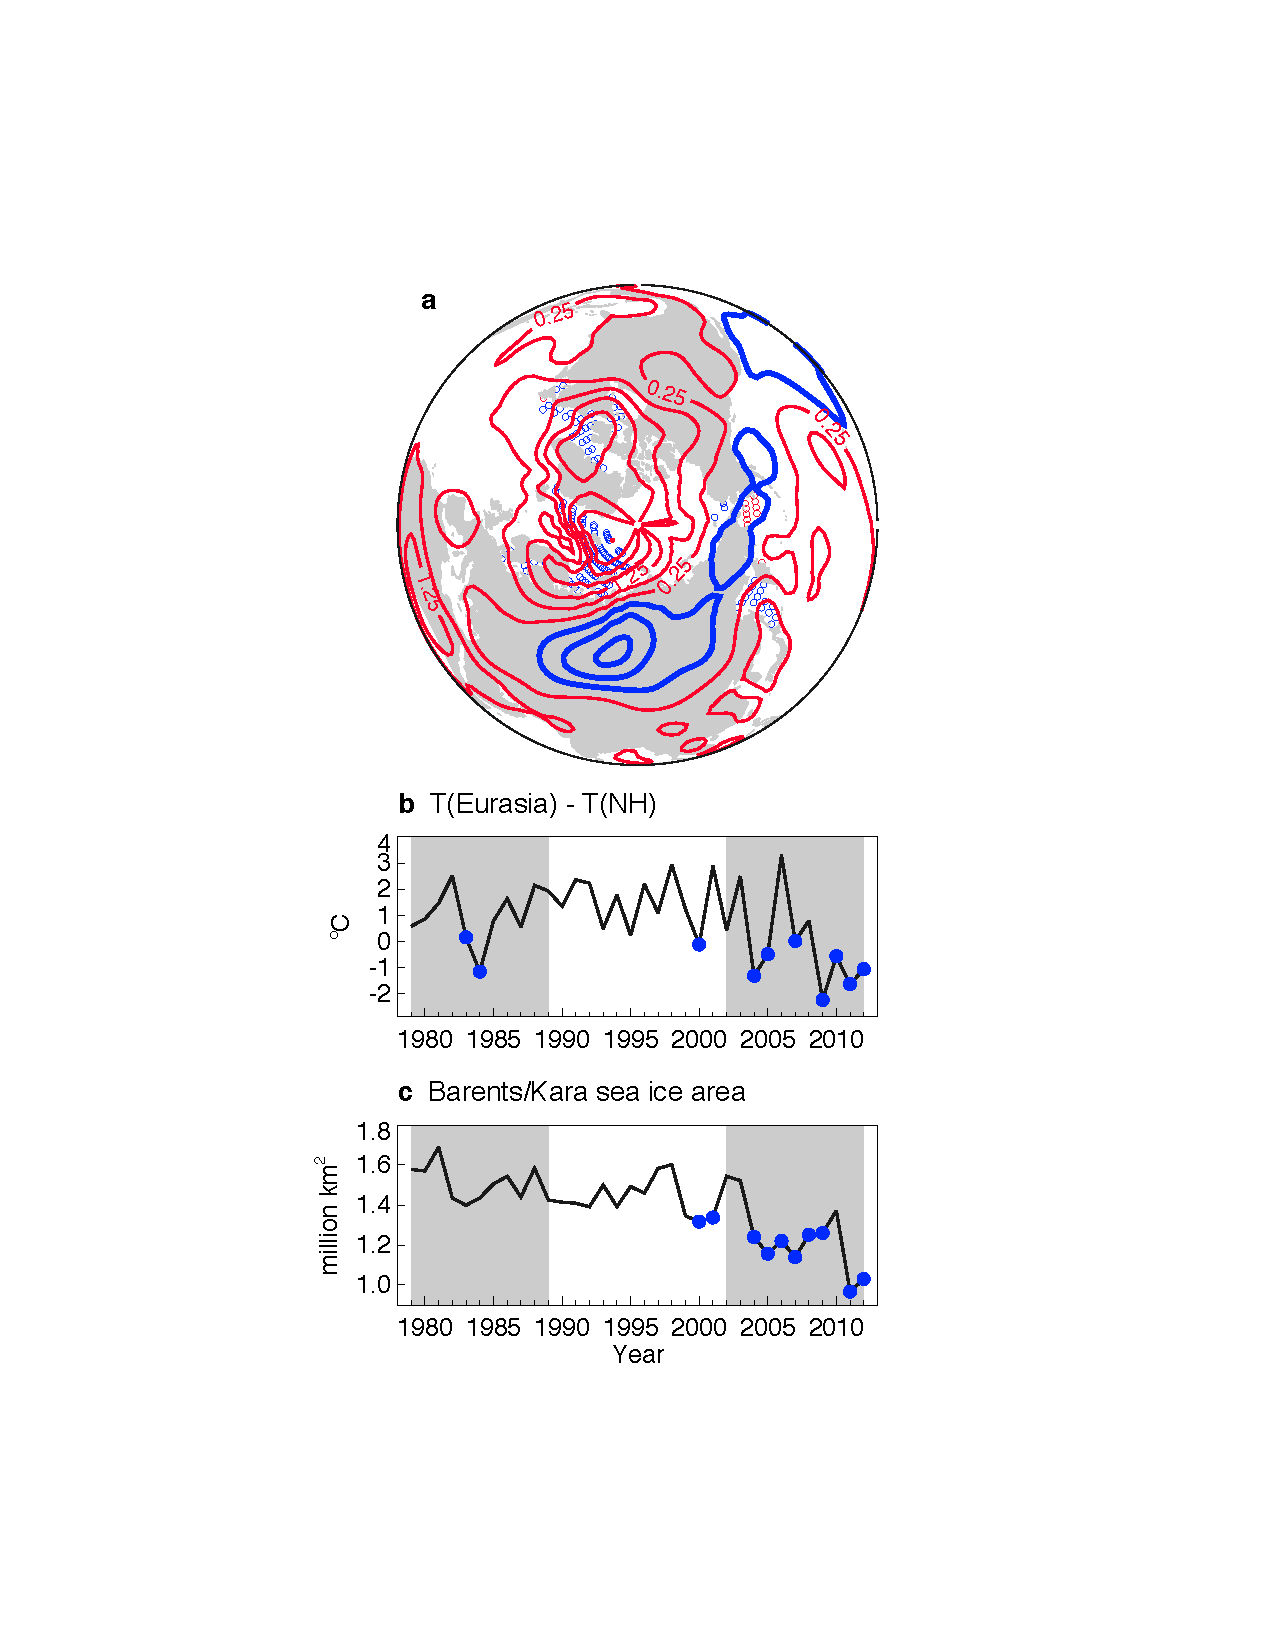
\includegraphics[width=19pc]{Word/Figure_1.pdf}
\caption{\textbf{Observed surface air temperature and sea ice concentration.} a.) Map of GIStemp winter surface air temperature anomalies as (2002-12) minus (1979-89) in contours. Contour interval is 0.5$^\circ$C with zero contour omitted. Stipling indicates regions of sea ice loss (blue) and gain (red) that are greater than 40\% in absolute terms. b.) Time series of Eurasian-averaged (35$^\circ$N - 60$^\circ$N, 40$^\circ$E - 120$^\circ$E) winter SAT with hemispheric (NH) winter temperature removed. Blue markers indicate the 10 most negative anomalies since 1979. c.) Time series of Barents-Kara Seas region (65$^\circ$N - 80$^\circ$N, 27$^\circ$E - 96$^\circ$E) winter sea ice area. Blue markers indicate the 10 lowest concentrations since 1979.
}
\label{fig:fig1} 
\end{figure}

\begin{figure}%[htbp] % the star afterwards makes it a one column fig in a 2-col document
\centering
\noindent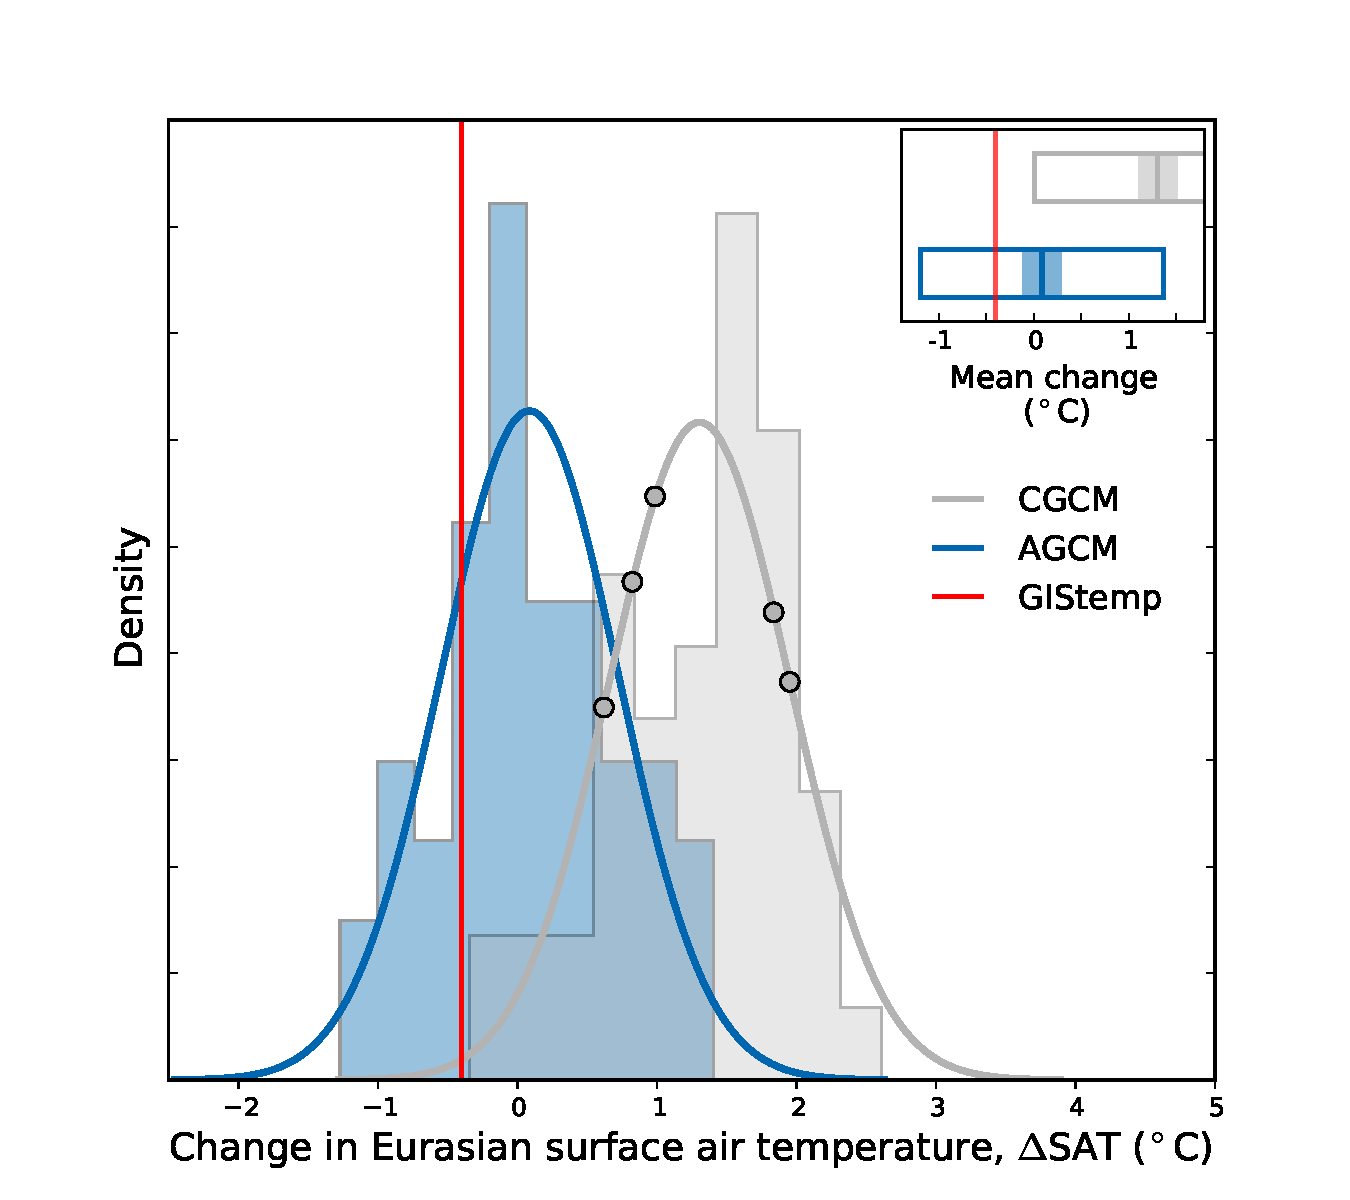
\includegraphics[width=25pc]{Word/Figure_2.pdf}
\caption{\textbf{Winter Eurasian surface air temperature (SAT) anomalies.} Histograms and associated probability distributions of winter Eurasian SAT anomalies (2002-12 minus 1979-89) sampled from the CGCM ensemble (gray) and anomalies sampled from the AGCM timeslice ensemble (blue). The red vertical line shows the observed anomaly computed from the GIStemp 1200km smoothed dataset. Gray circles indicate the Eurasian SAT anomalies in the 5 simulations whose Arctic sea ice concentration is used as boundary conditions to the AGCM ensemble. The inset is as the main panel but shows the probability distribution mean (line), 5-95\% confidence range on the mean (shading), and 5-95\% range of the probability distribution (box).
} % @@@ add: Filled markers indicate the present day period (2002-12) is significantly different from the past (1979-89) at the 90\% level using the Student’s T test of difference between two means. @@ Check confidence range: is it actually 2.5 - 97.5?
\label{fig:fig2} 
\end{figure}

\begin{figure}%[htbp] % the star afterwards makes it a one column fig in a 2-col document
\centering
\noindent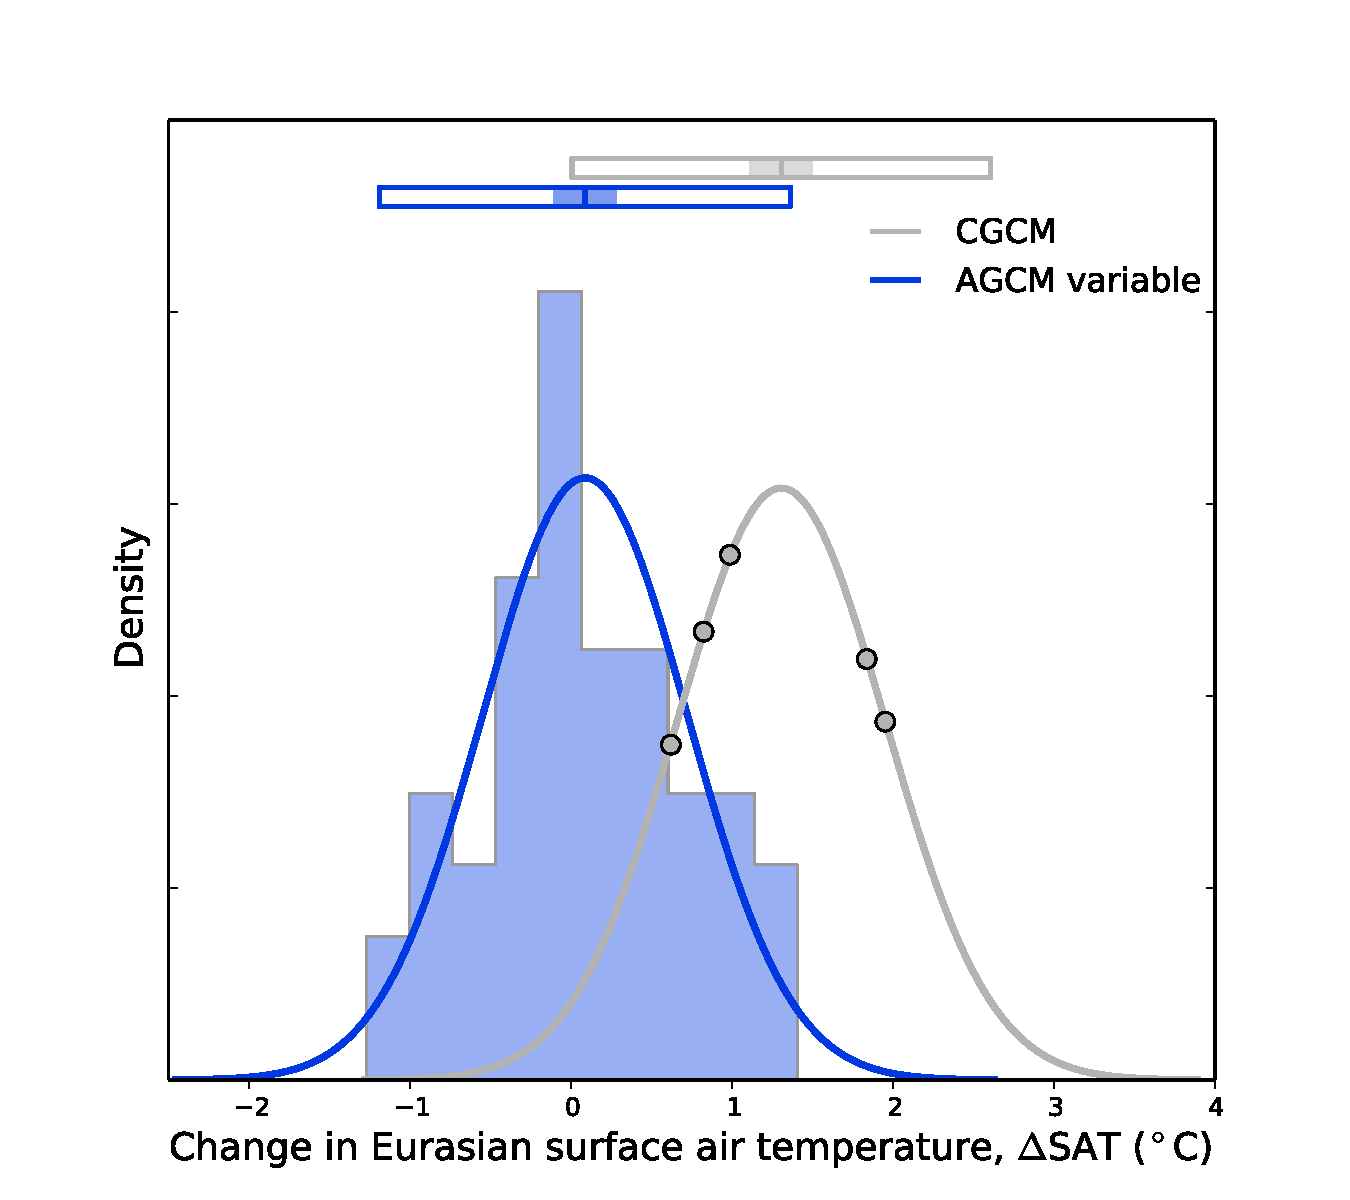
\includegraphics[width=35pc]{Word/Figure_3.pdf}
\caption{\textbf{Winter Barents/Kara 500 hPa geopotential height (Z500) anomalies versus winter Eurasian SAT anomalies.} Ellipses depict the 5-95\% confidence range of the relationship between anomalies in Barents/Kara Z500 (m) and associated anomalies in Eurasian SAT (oC) in the CGCM ensemble (dashed) and the AGCM ensemble (solid). Regression lines are shown for the CGCM (dashed) and AGCM (solid) ensembles. Plus markers show the value composited on the 10 smallest sea ice loss anomalies (red) and 10 largest sea ice loss anomalies (blue) in each ensemble. For both CGCM and AGCM, Barents/Kara Z500 composite anomalies are statistically different at the 95\% level (@@), but Eurasian SAT composite anomalies are not. The red circle indicates the observed value from ERA-Interim and GIStemp for Z500 and SAT, respectively. @@ADD 10-samp avg of NSIDC simulation?
}
\label{fig:fig3} 
\end{figure}

\begin{figure}%[htbp] % the star afterwards makes it a one column fig in a 2-col document
\centering
\noindent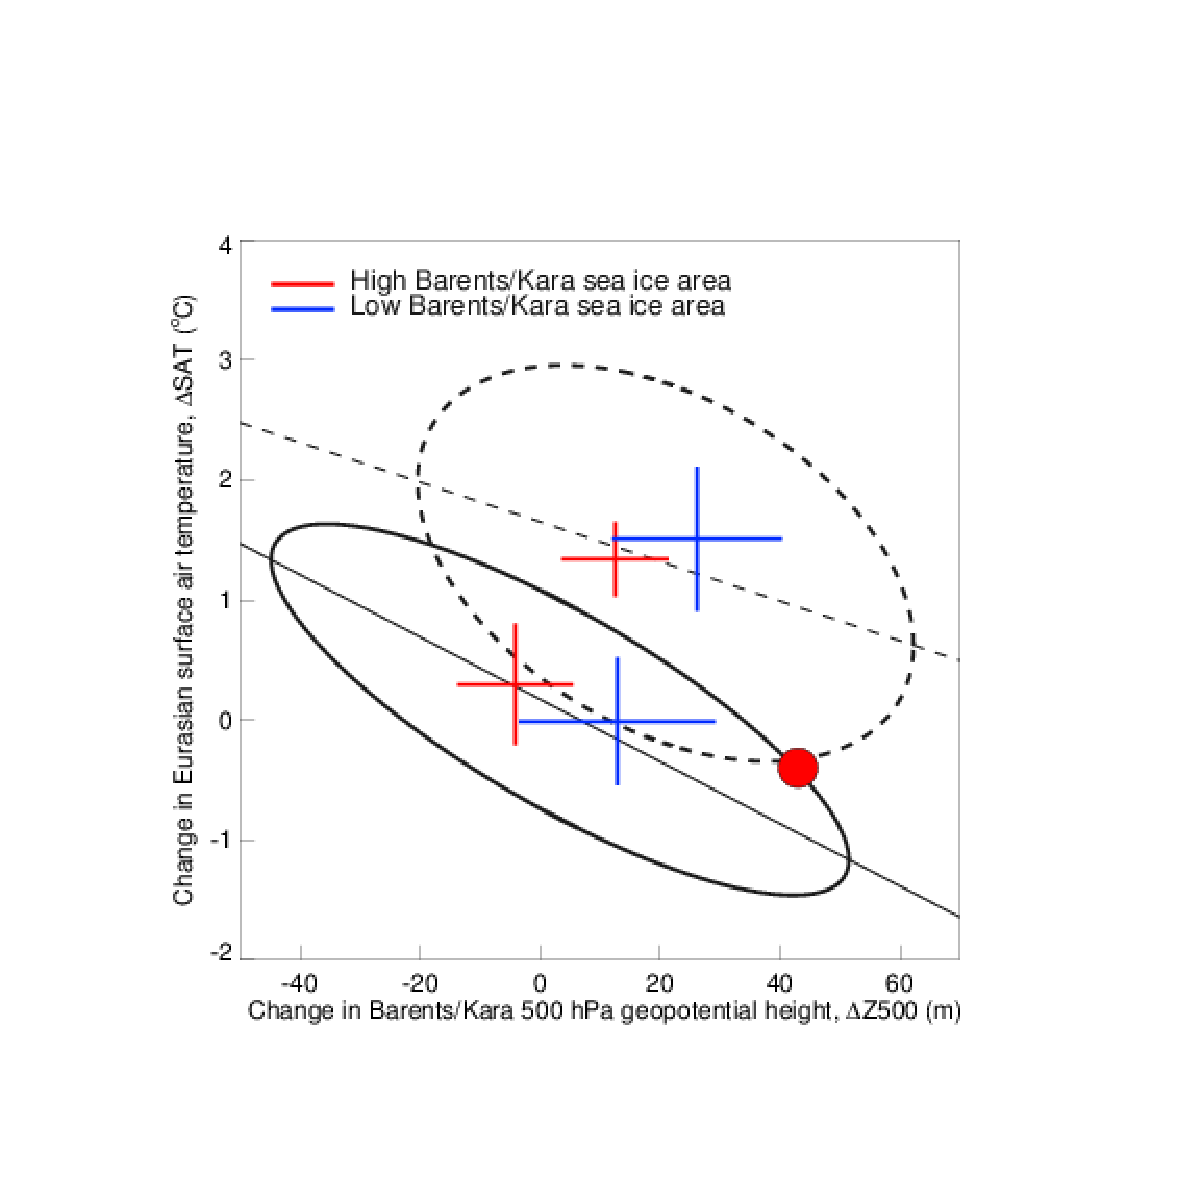
\includegraphics[width=39pc]{Word/Figure_4.pdf}
\caption{\textbf{Winter composites on Eurasian surface air temperature (Eur SAT), Barents/Kara sea ice concentration (BKS SIC), and Barents/Kara geopotential height at 500 hPa (BKS Z500.} Spatial patterns of change in surface air temperature (shading) and Z500 (contours) in CGCM associated with the a) ?low-high? (cold-warm) composite of Eur SAT, b) ?low-high? composite of BKS SIC, and c) ?high-low? composite of BKS Z500. Z500 contour interval @@@. d-f) show regional average anomalies, indicated on the y-axis, associated with the 3 composites shown in a-c. d) The change in SAT (oC) averaged over Eurasia (35oN ? 60oN, 40oE ? 120oE) associated with the ?low-high? composite of BKS SIC (left column; map shown in a.), and associated with the ?high-low? composite of BKS Z500 (right column; map shown in c.) for each of the ensembles (CGCM, Preindustrial, AGCM). e) and f) are as d) but showing the change in SIC in the Barents/Kara Seas (\%) and change in Z500 (m) averaged over the Barents/Kara seas, respectively, and only show anomalies for composites on fields other than itself..
}
\label{fig:fig4} 
\end{figure}

\begin{figure}%[htbp] % the star afterwards makes it a one column fig in a 2-col document
\centering
\noindent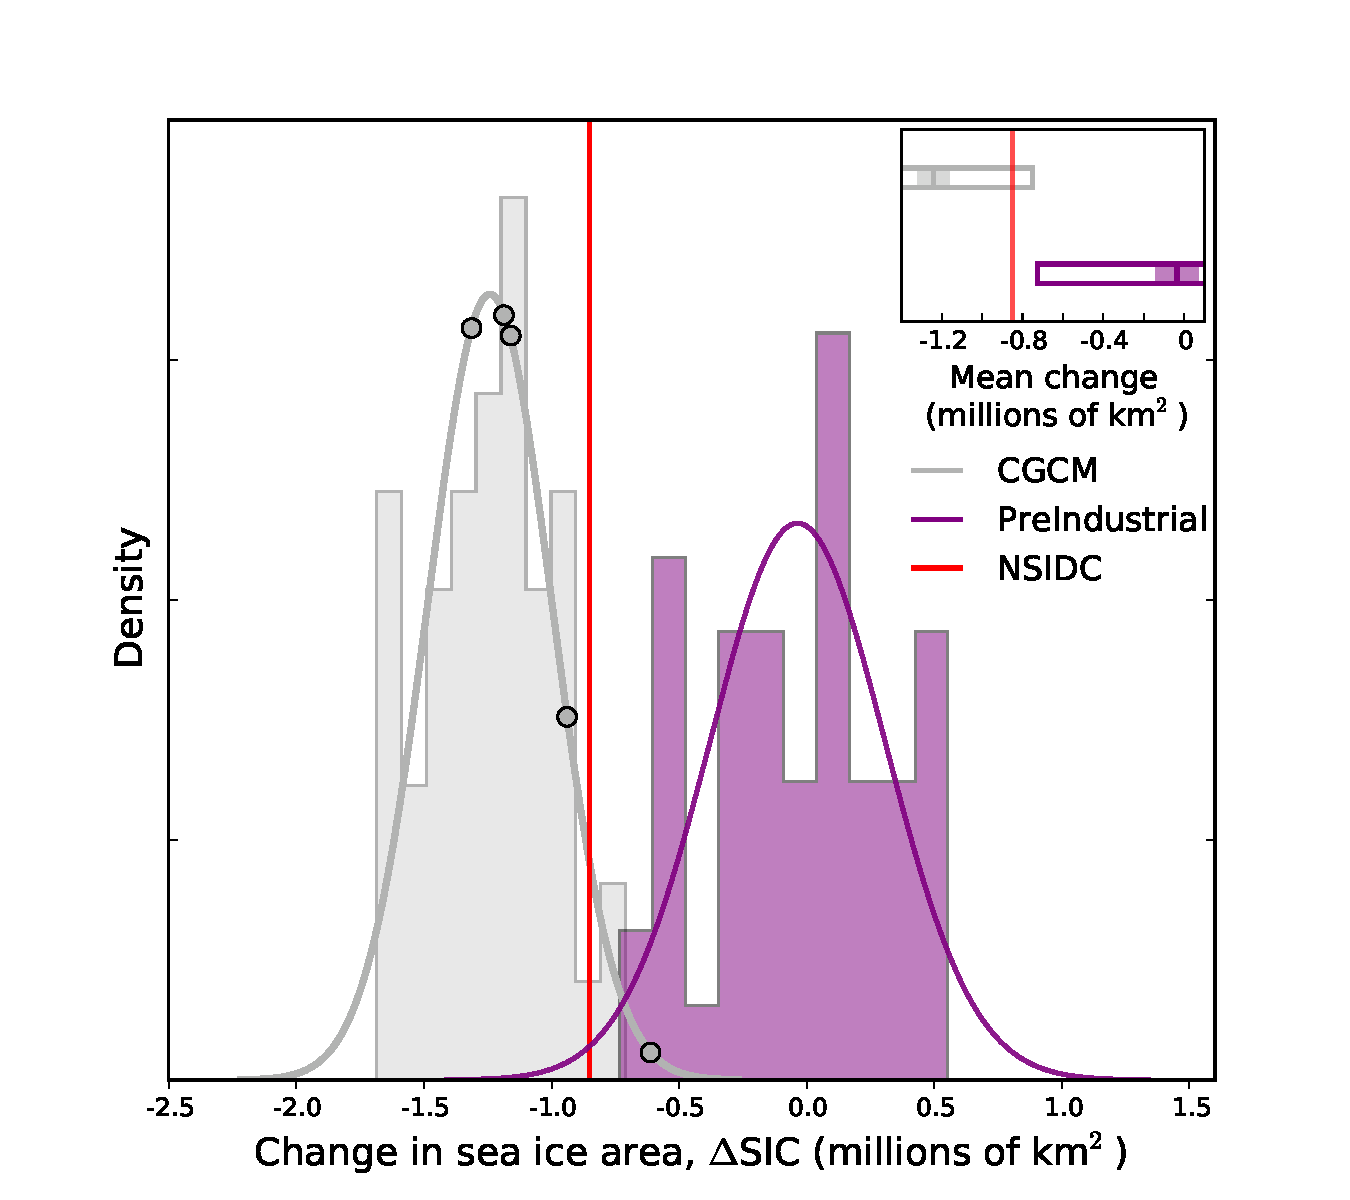
\includegraphics[width=39pc]{Word/SuppFig_1.pdf}
\caption{\textbf{Winter Arctic sea ice area (SIA) anomalies.} Histograms and associated probability distributions of winter Arctic SIA anomalies (2002-12 minus 1979-89) sampled from the CGCM ensemble (gray) and anomalies sampled from the Preindustrial ensemble (purple). The red vertical line shows the observed anomaly computed from the National Sea Ice Data Center (NSIDC) bootstrap dataset. Gray circles indicate the Arctic SIA anomalies in the 5 simulations whose Arctic sea ice concentration is used as boundary conditions to the AGCM ensemble. The inset is as the main panel but shows the probability distribution mean (line), 5-95\% confidence range on the mean (shading), and 5-95\% range of the probability distribution (box).
} 
\label{fig:supfig1} 
\end{figure}

%% Put the bibliography here, most people will use BiBTeX in
%% which case the environment below should be replaced with
%% the \bibliography{} command.

%\begin{thebibliography}{1}
%\end{thebibliography}
\newpage

%\bibliographystyle{ametsoc}
\bibliography{allrefs}





% ~/bibtexrefs/allrefs  == this is version controlled now, but will have to just copy into current dir?


%% Here is the endmatter stuff: Supplementary Info, etc.
%% Use \item's to separate, default label is "Acknowledgements"

\begin{addendum}
\item[Acknowledgements] 
\item[Author Contributions] 
 \item[Competing Interests] The authors declare that they have no competing financial interests.
\item[Correspondence] Correspondence and requests for materials should be addressed to K.E.M.~(email: kemccusk@uvic.ca).
\end{addendum}

%%
%% TABLES
%%
%% If there are any tables, put them here.
%%

\end{document}
